%!TEX root = thesis.tex

\chapter{Evaluation of the Framework}
\label{chp:Evaluation}

This chapter presents the empirical evaluation of the \gls{tinylcm} framework, conducted according to the refined experimental design detailed in Section~\ref{sec:FrameworkEvaluationMethodology}. The evaluation is structured into two primary phases: Phase 1 assesses the performance overhead introduced by \gls{tinylcm} components, and Phase 2 validates the framework's functional drift detection capabilities. The results are analyzed to test the hypotheses H$_1$, H$_2$, and H$_3$ formulated in Section~\ref{ssec:refined_experimental_design_final}. Finally, a cross-phase discussion synthesizes the findings, and potential threats to the validity of these results are considered.

~\\
\vfill
\minitoc
\clearpage

\section{Experimental Setup Implementation}
\label{sec:exper-setup_implementation}

The experiments were conducted in a controlled laboratory environment to ensure consistency and reproducibility, as described in Section~\ref{ssec:refined_experimental_design_final}. Figure~\ref{fig:exp_setup_photo} illustrates the physical setup used for data collection. Key aspects included fixed camera positioning (\SI{15}{\centi\meter} to object surface), defined object placement markers, and controlled lighting conditions (dual artificial light sources, minimized ambient light) to reduce environmental variability.

\begin{figure}[htbp]
  \centering
  \includegraphics[width=.55\linewidth]{figs/evaluation/exp_setup.png}
  \caption[Photograph of the Controlled Experimental Setup]{Physical setup for the controlled experiments, showing the Raspberry Pi Zero 2W with camera module, consistent object placement area with markers, and controlled lighting.}
  \label{fig:exp_setup_photo}
\end{figure}

\section{Phase 1 – Performance Overhead Assessment}
\label{sec:phase1_results_overhead}

This phase aimed to quantify the computational and memory overhead introduced by the \gls{tinylcm} framework components. The three staged configurations (Baseline, \gls{tinylcm} (no drift), \gls{tinylcm} (with drift detection)) were executed in five independent runs each. After excluding the warm-up period, a substantial number of measurements ($N$) were collected for each configuration.


\subsection{Resource Utilization and Inference Latency}
\label{ssec:phase1_combined_analysis_latency}

Table~\ref{tab:performance_summary_values_eval} provides a summary of the key performance metrics. It shows the descriptive statistics (mean and standard deviation) calculated across all individual measurements collected from the five independent runs for each configuration. For a more detailed temporal view, time series visualizations of the CPU, memory, and latency data for each configuration are available in Appendix~\ref{app:eval-data}.

\begin{table}[htbp]
    \centering
    \caption[Descriptive Statistics of Performance Metrics from All Measurements (Phase 1)]{Descriptive statistics for key performance metrics, calculated over all measurements ($N$) from the five independent runs.}
    \label{tab:performance_summary_values_eval}
    \footnotesize
    \begin{tabularx}{\linewidth}{@{}X c r@{$\pm$}l r@{$\pm$}l r@{$\pm$}l@{}}
        \toprule
        \textbf{Configuration} & \textbf{$N$} & \multicolumn{2}{c}{CPU Usage (\%)} & \multicolumn{2}{c}{Memory (MB)} & \multicolumn{2}{c}{Latency (ms)} \\
        \midrule
        Baseline \gls{tfl} & 1306 & 3.33 & 1.73 & 174.55 & 0.24 & 357.68 & 1.91 \\
        \gls{tinylcm} (no drift) & 1089 & 5.39 & 3.03 & 229.93 & 1.65 & 419.66 & 4.36 \\
        \gls{tinylcm} (drift detection) & 873 & 4.10 & 3.10 & 203.92 & 9.58 & 435.60 & 43.74 \\
        \bottomrule
    \end{tabularx}
\end{table}

Observing Table~\ref{tab:performance_summary_values_eval} and the corresponding visualizations:
\begin{itemize}[noitemsep, topsep=0pt]
    \item \textit{CPU Usage:} The Baseline configuration showed a mean CPU usage of $3.33 \pm 1.73$\%. This increased to $5.39 \pm 3.03$\% for the \gls{tinylcm} (no drift) configuration. With drift detection enabled, the mean CPU usage was $4.10 \pm 3.10$\%.
    \item \textit{Memory Usage:} Memory usage increased from a mean of $174.55 \pm 0.24$\,\si{\mega\byte} for the Baseline to $229.93 \pm 1.65$\,\si{\mega\byte} for \gls{tinylcm} (no drift). The \gls{tinylcm} (drift detection) configuration had a mean memory of $203.92 \pm 9.58$\,\si{\mega\byte}.
    \item \textit{Inference Latency:} Mean inference latency increased from $357.68 \pm 1.91$\,\si{\milli\second} for the Baseline to $419.66 \pm 4.36$\,\si{\milli\second} for \gls{tinylcm} (no drift), and further to $435.60 \pm 43.74$\,\si{\milli\second} for the full framework. The significantly larger standard deviation for the drift detection configuration suggests the presence of high-latency outliers, likely corresponding to the execution of the drift check itself.
\end{itemize}

While Table~\ref{tab:performance_summary_values_eval} provides a global overview of all collected data points, the subsequent hypothesis testing relies on treating each of the five experimental runs as an independent sample. This approach is methodologically crucial to avoid pseudo-replication and to validly assess the variability between runs. Therefore, the statistical tests in Section~\ref{ssec:phase1_hyp_tests} are performed on the distributions of the $n=5$ aggregate values. The distributions of these aggregate values are visualized through boxplots in Figure~\ref{fig:performance_boxplots_eval} and histograms in Figure~\ref{fig:performance_histograms_density_eval}.

\begin{figure}[htbp]
  \centering
  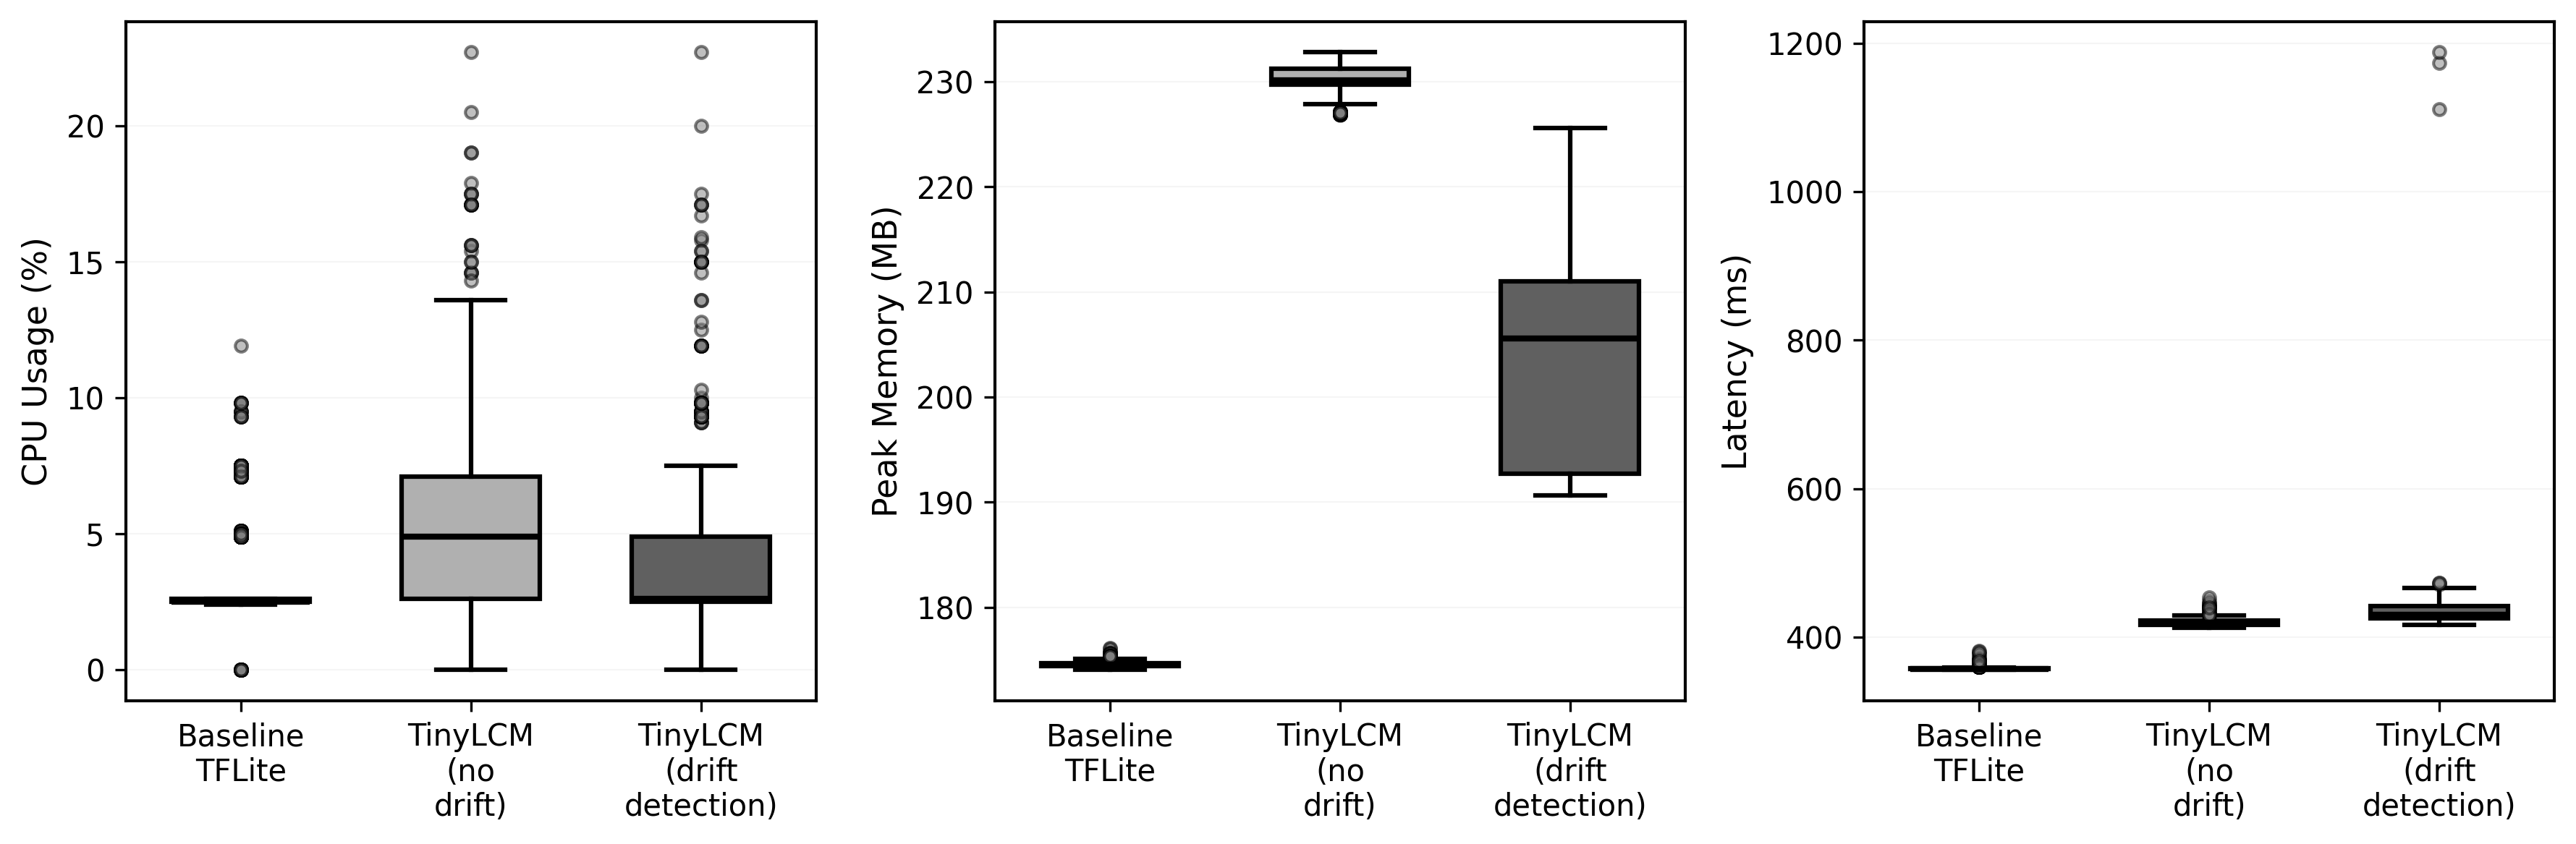
\includegraphics[width=.98\linewidth]{figs/evaluation/boxplots_N5.png}
  \caption[Boxplot Analysis of Aggregated Performance Metrics]{Comparative boxplot analysis of CPU usage (\%), memory (\si{\mega\byte}), and latency (\si{\milli\second}) for the three configurations, based on the runs per configuration. Individual data points are overlaid.}
  \label{fig:performance_boxplots_eval}
\end{figure}

\begin{figure}[htbp]
  \centering
  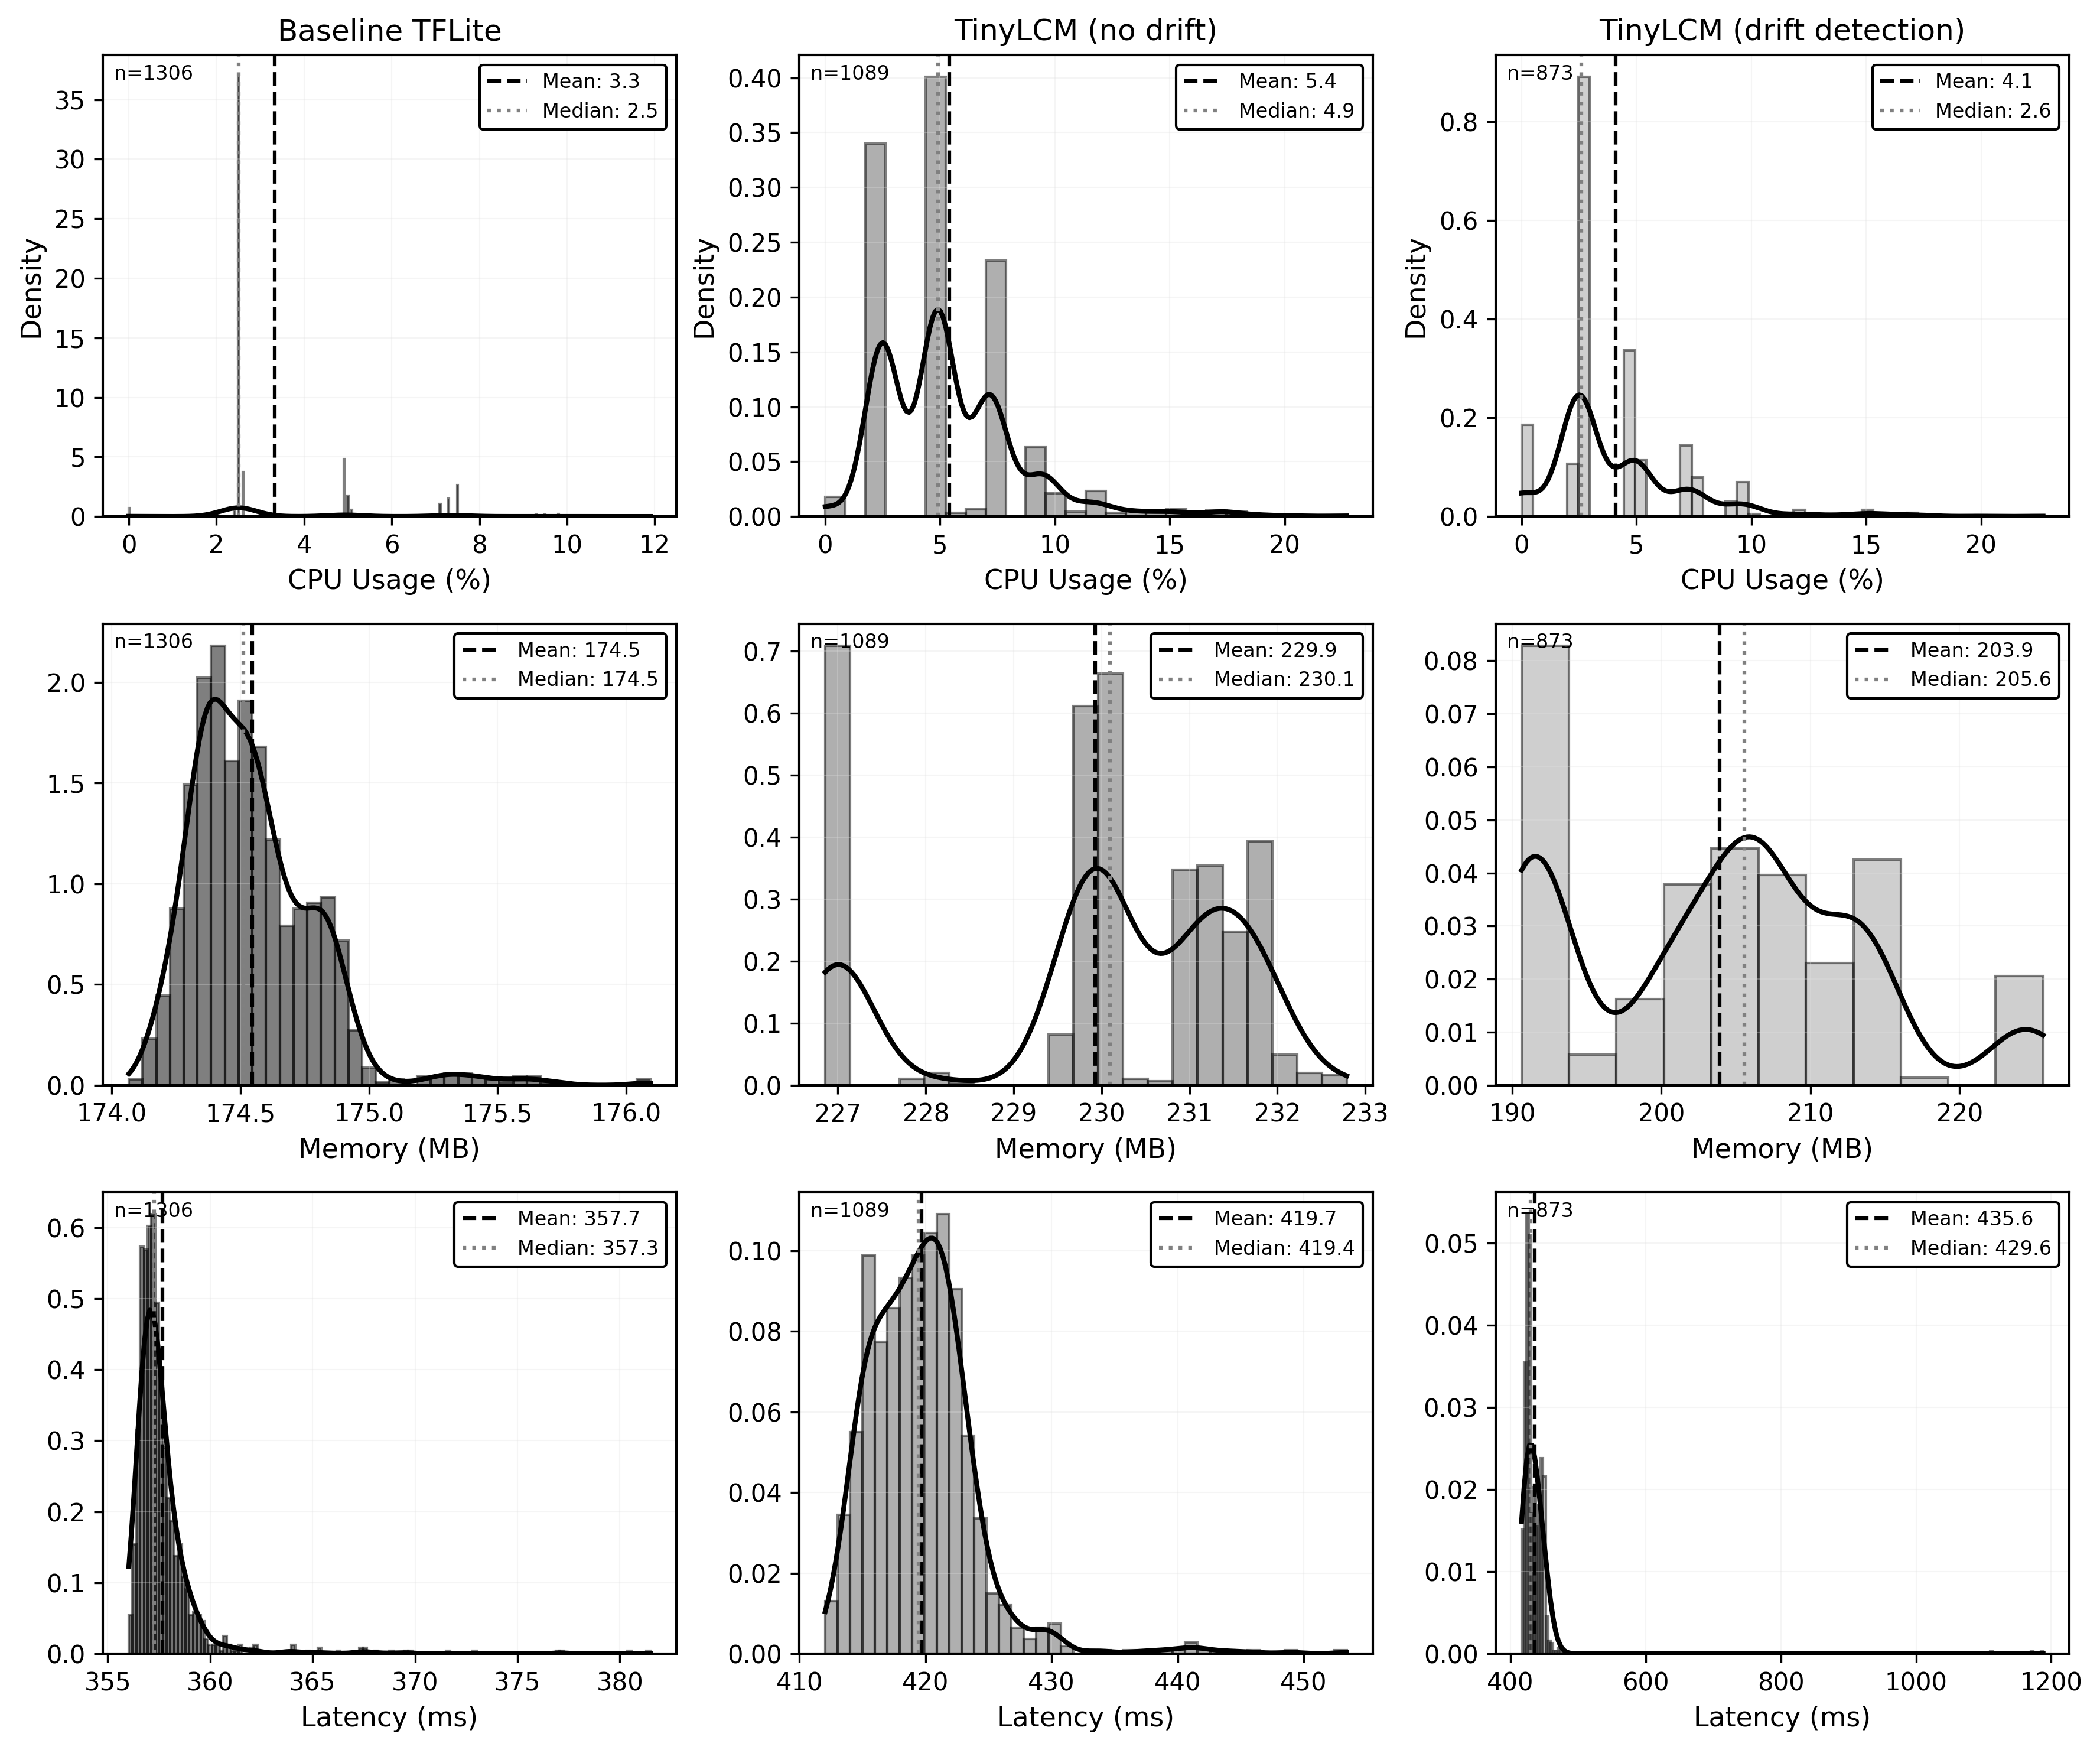
\includegraphics[width=.98\linewidth]{figs/evaluation/histograms_density_N5.png}
  \caption[Histograms and Kernel Density Estimates of Aggregated Performance Metrics]{Distributions of CPU usage (\%), memory (\si{\mega\byte}), and latency (\si{\milli\second}) for the three configurations, based on the runs per configuration. Histograms are overlaid with kernel density estimates and a vertical line indicating the mean.}
  \label{fig:performance_histograms_density_eval}
\end{figure}

\subsection{Hypothesis Testing (H$_1$ and H$_2$)}
\label{ssec:phase1_hyp_tests}

Prior to hypothesis testing, the full datasets for each metric and configuration (N > 800) were assessed for normality using the Shapiro-Wilk test. The tests confirmed that all examined distributions significantly deviate from normality (all $p \ll 0.001$). Consequently, non-parametric one-sample Wilcoxon signed-rank tests were used to evaluate H$_1$ and H$_2$ against their defined thresholds. The results are summarized in Table~\ref{tab:h1_h2_test_results}.

As shown in Table~\ref{tab:h1_h2_test_results}, all tests yielded highly significant results ($p \ll 0.001$), confirming that the observed performance metrics are well within their predefined acceptable limits. The latency overhead for both \gls{tinylcm} configurations was significantly below 50\%. Likewise, the CPU and memory usage were significantly below their respective thresholds. Therefore, both \textbf{H$_1$ and H$_2$ are accepted}.

\begin{table}[htbp]
    \centering
    \caption[Summary of Hypothesis Test Results for H$_1$ and H$_2$]{Results of the one-sided one-sample Wilcoxon signed-rank tests for H$_1$ and H$_2$.}
    \label{tab:h1_h2_test_results}
    \footnotesize
    \begin{tabularx}{\linewidth}{@{}l l X r c r@{}}
        \toprule
        \textbf{Hypothesis} & \textbf{Metric} & \textbf{Configuration} & \textbf{Statistic (W)} & \textbf{Threshold} & \textbf{$p$-value} \\
        \midrule
        \textbf{H$_1$} & Latency Overhead & \gls{tinylcm} (no drift) & 0.0 & < 50\% & $5.10\times10^{-180}$ \\
                      &                   & \gls{tinylcm} (drift detection) & 2616.0 & < 50\% & $6.53\times10^{-141}$ \\
        \addlinespace
        \textbf{H$_2$} & CPU Usage & \gls{tinylcm} (no drift) & 0.0 & < 50\% & $2.17\times10^{-180}$ \\
                      &           & \gls{tinylcm} (drift detection) & 0.0 & < 50\% & $1.44\times10^{-146}$ \\
        \addlinespace
        \textbf{H$_2$} & Memory & \gls{tinylcm} (no drift) & 0.0 & < 256 MB & $5.10\times10^{-180}$ \\
                      &        & \gls{tinylcm} (drift detection) & 0.0 & < 256 MB & $8.57\times10^{-145}$ \\
        \bottomrule
    \end{tabularx}
\end{table}

To compare the performance between configurations, the Mann-Whitney U test was used, with Cliff's delta ($\delta$) as the measure of effect size. The results are summarized in Table~\ref{tab:phase1_mannwhitney_results}. It demonstrate that all pairwise comparisons between the configurations yielded statistically significant differences. The addition of the \gls{tinylcm} pipeline (S1) to the baseline (S0) resulted in a medium increase in CPU usage and a large increase in memory and latency. Adding drift detection (S2) also caused a significant increase in latency and memory compared to baseline, though the effect on CPU usage was negligible.
Comparing the two \gls{tinylcm} configurations directly, the full framework with drift detection (S2) exhibited significantly higher latency (large effect) but significantly lower CPU usage (small effect) and memory usage (large effect) than the pipeline without drift detection (S1). This counterintuitive result regarding CPU and memory is further explored in the methodological reflection below.

\begin{table}[htbp]
  \centering
  \caption[Mann-Whitney U Test Results for Phase 1 Performance Metrics]{Mann-Whitney U test results and Cliff's delta effect sizes for comparing independent configurations. S1 = \gls{tinylcm} (no drift), S2 = \gls{tinylcm} (with drift detection), S0 = Baseline. Effect size interpretation: L=Large, M=Medium, S=Small, N=Negligible.}
  \label{tab:phase1_mannwhitney_results}
  \footnotesize
  \setlength{\tabcolsep}{3pt} 
  \begin{tabularx}{\linewidth}{@{}X r c r@{}} 
    \toprule
    \textbf{Metric (Comparison Pair)} & \textbf{Statistic ($U$)} & \textbf{$p$-value} & \textbf{Cliff's $\delta$ (Interpretation)} \\ 
    \midrule
    CPU Usage (\%) (S1 vs. S0)      & $997726.5$ & $4.25\times10^{-70}$ & $+0.40$ (M) \\
    CPU Usage (\%) (S2 vs. S0)      & $636664.0$ & $4.09\times10^{-7}$ & $+0.12$ (N) \\ 
    CPU Usage (\%) (S2 vs. S1)      & $353119.0$ & $5.16\times10^{-23}$ & $-0.26$ (S) \\ 
    \addlinespace
    Memory (\si{\mega\byte}) (S1 vs. S0)    & $1422234.0$ & $0.0$ & $+1.0$ (L) \\ 
    Memory (\si{\mega\byte}) (S2 vs. S0)    & $1140138.0$ & $0.0$ & $+1.0$ (L) \\
    Memory (\si{\mega\byte}) (S2 vs. S1)    & $0.0$       & $0.0$ & $-1.0$ (L) \\
    \addlinespace
    Latency (\si{\milli\second}) (S1 vs. S0)   & $1422234.0$ & $0.0$ & $+1.0$ (L) \\
    Latency (\si{\milli\second}) (S2 vs. S0)   & $1140138.0$ & $0.0$ & $+1.0$ (L) \\
    Latency (\si{\milli\second}) (S2 vs. S1)   & $877097.0$  & $1.08\times10^{-227}$ & $+0.85$ (L) \\
    \bottomrule
  \end{tabularx}
\end{table}

\begin{MyBox}{Methodological Reflection on Experimental Run Order and Observed Variances}
    During the execution of the Phase 1 performance experiments, an observation was made regarding resource utilization that warrants reflection. As indicated in Table~\ref{tab:performance_summary_values_eval} and confirmed by the statistical tests in Table~\ref{tab:phase1_mannwhitney_results}, the \gls{tinylcm} (no drift) configuration (S1) exhibited significantly higher memory ($229.93$\,\si{\mega\byte}) and CPU usage ($5.39\%$) compared to the \gls{tinylcm} (with drift detection) configuration (S2) (memory: $203.92$\,\si{\mega\byte}, CPU: $4.10\%$). This is counterintuitive, as S2 performs strictly more operations than S1.

    While the Python code for both configurations is functionally correct, this specific pattern might be partly attributable to the experimental execution history. The $n=5$ runs for each configuration block (Baseline, S1, S2) were performed as distinct sets, with system restarts intended between the blocks. However, it was noted that the S1 runs were conducted at an earlier stage of the overall experimental campaign, possibly involving more iterative adjustments in the setup or more intensive system activity immediately preceding or during some of those runs compared to the later S2 runs. Such historical factors, even with restarts, could potentially lead to subtle differences in the system's baseline state (e.g., OS caching, background process activity accumulated over time, or even minor variations in ambient temperature affecting the hardware) that might influence resource measurements, especially for memory and CPU.

    Ideally, to completely mitigate such potential temporal or historical biases, a more rigorous protocol would involve a fully randomized or counterbalanced execution order of the three configurations across the 5 ``runs'' (where each run contains one instance of each configuration), along with complete system state resets (e.g., reflashing the OS) before each run.
    
    This reflection does not invalidate the primary findings regarding the overall overhead compared to baseline or the feasibility within resource constraints (H$_1$, H$_2$). However, it provides important context for interpreting fine-grained differences between the two \gls{tinylcm} configurations and underscores a potential subtle threat to internal validity, further discussed in Section~\ref{sec:result_level_threats_validity}.
\end{MyBox}

\subsection{Latency Breakdown}
\label{ssec:phase1_latency_breakdown}

To understand the contributions of different processing stages to the overall inference latency of the \gls{tinylcm} configurations, a detailed breakdown was performed. Table~\ref{tab:latency_components_summary} presents the mean processing times and their percentage contribution to the total latency for each measured component within the ``TinyLCM (no drift)'' and ``TinyLCM (drift detection)'' pipelines. These statistics are derived from aggregating measurements across all processed frames from the $n=5$ independent runs for each configuration, as detailed in the.

\begin{table}[htbp]
    \centering
    \caption[Mean Processing Time of Latency Components for \gls{tinylcm} Configurations (Phase 1)]{Mean processing time and percentage of total latency for each measured component in the \gls{tinylcm} configurations.}
    \label{tab:latency_components_summary}
    \footnotesize
    \begin{tabularx}{\linewidth}{@{}X rr rr@{}} % X für Komponenten, dann 2x rr für Wertepaare
        \toprule
        \textbf{Component} & \multicolumn{2}{c}{\textbf{TinyLCM (no drift)}} & \multicolumn{2}{c}{\textbf{TinyLCM (drift detection)}} \\
        \cmidrule(lr){2-3} \cmidrule(lr){4-5} % Linien unter den Konfigurationsnamen
         & \multicolumn{1}{r}{Mean (\si{\milli\second})} & \multicolumn{1}{r}{(\% Total)} & \multicolumn{1}{r}{Mean (\si{\milli\second})} & \multicolumn{1}{r}{(\% Total)} \\
        \midrule
        Feature Extraction (incl. Base Model, PCA, Scale)$^{\text{a}}$ & 353.71 & 84.29\% & 353.98 & 81.26\% \\
        KNN Inference$^{\text{b}}$ & 65.94 & 15.71\% & 66.42 & 15.25\% \\
        Drift Check & 0.00 & 0.00\% & 1.73 & 0.40\% \\
        Other (Preprocessing, Pipeline Overhead) & 0.01 & 0.00\% & 13.47 & 3.09\% \\
        \midrule
        \textbf{Total Measured Latency} & \textbf{419.66} & \textbf{100\%} & \textbf{435.60} & \textbf{100\%} \\
        \bottomrule
    \end{tabularx}
\end{table}

Table~\ref{tab:latency_components_summary} details the latency contributions. The ``Feature Extraction'' component, which encompasses the execution of the base \gls{tfl} model along with subsequent feature processing steps (such as PCA and scaling), consistently consumes the largest portion of time, averaging approximately $353.71$\,\si{\milli\second} ($84.29\%$) for the ``TinyLCM (no drift)'' configuration and $353.98$\,\si{\milli\second} ($81.26\%$) for the ``TinyLCM (drift detection)'' configuration. This indicates that the core model inference and primary feature derivation dominate the processing time.

The ``KNN Inference'' stage, responsible for the \gls{knn} search and classification based on the processed features, adds a mean of $65.94$\,\si{\milli\second} ($15.71\%$) in the ``no drift'' configuration and $66.42$\,\si{\milli\second} ($15.25\%$) when drift detection is active. The similarity in KNN inference time between the two \gls{tinylcm} configurations is expected, as the core KNN lookup process remains the same.

The ``Drift Check'' component, only active in the ``TinyLCM (drift detection)'' configuration, introduces a mean overhead of $1.73$\,\si{\milli\second}, which constitutes only $0.40\%$ of the total latency for that configuration. This demonstrates that the direct computational cost of the Page-Hinkley test and associated logic for the drift check itself is minimal.

Interestingly, the ``Other (Preprocessing, Pipeline Overhead)'' category shows a notable difference. For the ``TinyLCM (no drift)'' configuration, this overhead is negligible ($0.01$\,\si{\milli\second}). However, for the ``TinyLCM (drift detection)'' configuration, it averages $13.47$\,\si{\milli\second}, accounting for $3.09\%$ of the total latency. This suggests that enabling the drift detection mechanism introduces some additional, unmeasured overhead within the overall pipeline orchestration or data handling steps that occur between the explicitly timed main components. This could include, for example, managing data flow to the drift monitor, conditional checks, or state updates related to the drift detection status, even if the drift check calculation itself is fast. This ``Other'' overhead, when combined with the direct ``Drift Check'' time, largely explains the overall mean latency difference observed between the ``no drift'' ($419.66$\,\si{\milli\second}) and ``drift detection'' ($435.60$\,\si{\milli\second}) configurations as reported in Table~\ref{tab:performance_summary_values_eval}.

\begin{MyBox}{Subjective Interpretation of Latency Results}
	The observed inference latencies, particularly for the \gls{tinylcm} configurations (approx. 420-436\,\si{\milli\second}), correspond to a processing rate of roughly 2.3 frames per second. While acceptable for some near real-time applications, this is relatively high for others demanding faster responses. This latency is influenced by the choice of the MobileNetV2 base model and the Python implementation of \gls{tinylcm}. MobileNetV2 was selected for this study due to its ready availability and straightforward integration after initial attempts with more complex models like EfficientNet Lite encountered compilation and deployment challenges on the target platform. Future work could explore further model optimization or the use of different base architectures to potentially reduce this baseline latency.
\end{MyBox}

\section{Phase 2 – Drift Detection Validation}
\label{sec:phase2_results_drift}

This phase aimed to validate the functional drift detection capabilities of the \gls{tinylcm} framework. The core objective was to test whether the system could produce a statistically significant response to untrained objects. The ground truth for drift periods was determined by analyzing the prediction logs to identify the exact timestamps when untrained objects were presented.

\subsection{Drift Alarm Timelines}
\label{ssec:phase2_alarm_timelines}

Figures~\ref{fig:timeline-exp1_s1} and \ref{fig:timeline-exp2_s2} illustrate the prediction timelines and the occurrences of drift alarms generated by the \texttt{KNNDistanceMonitor} for Scenario 1 and Scenario 2, respectively.

\begin{figure}[htbp]
  \centering
  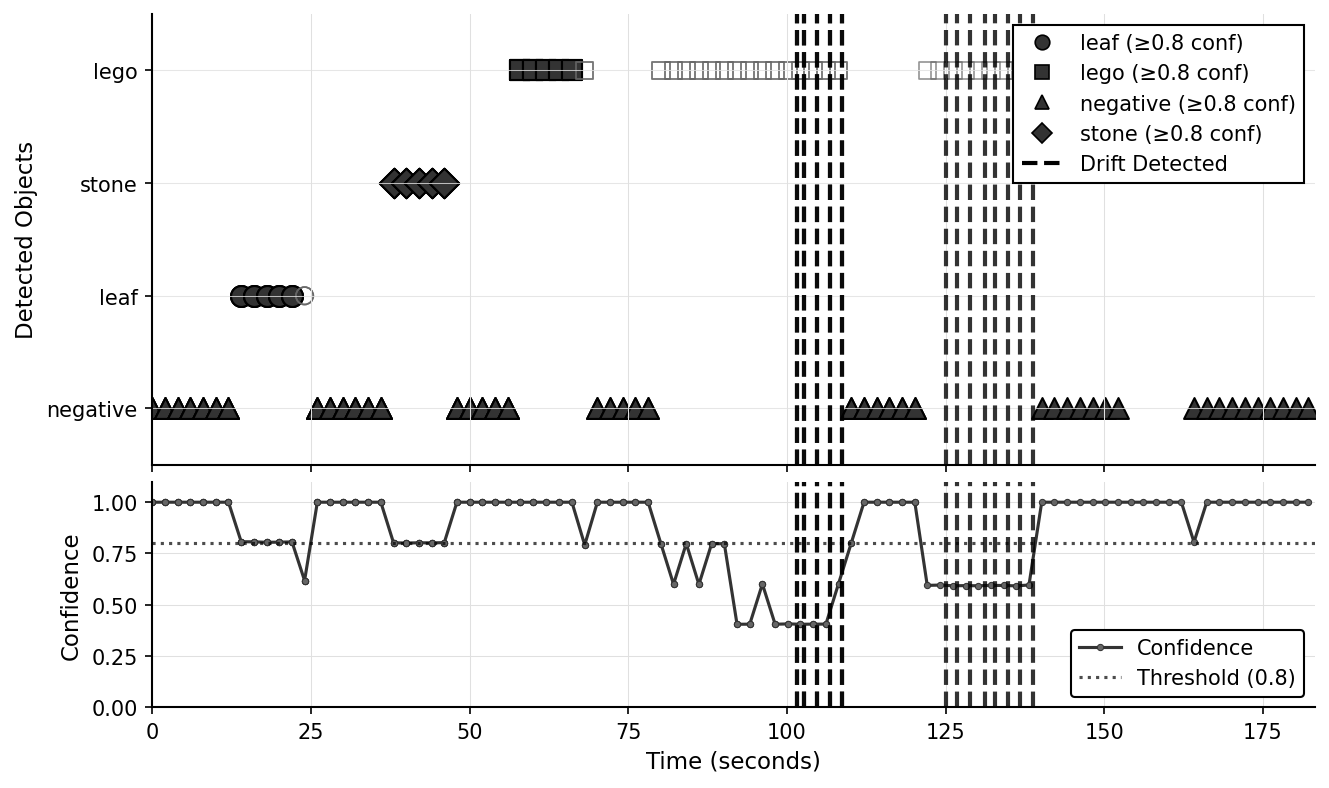
\includegraphics[width=.98\linewidth]{figs/evaluation/drift_coin_ball_timeline.png}
  \caption[Drift Prediction Timeline for Scenario S1 (Dual Drift)]{Prediction timeline and drift alarms for Scenario S1 (Dual Drift). Grey squares indicate the predicted class (y-axis) at each two-second interval. Dashed vertical lines mark drift alarms from the \texttt{KNNDistanceMonitor}. The sequence includes presentation of known classes and two novel drift objects (``ball'', ``coin'').}
  \label{fig:timeline-exp1_s1}
\end{figure}

Following the detection of these drift events, \gls{tinylcm}'s \texttt{SyncClient}, if active and connected, would package relevant information, including images of the objects causing the drift, for transmission to TinySphere. Figures~\ref{fig:drift-image-ball_s1} and \ref{fig:drift-image-coin_s1} show examples of such drift images.

\begin{figure}[htbp]
    \centering
    \begin{subfigure}{0.49\textwidth}
        \centering
        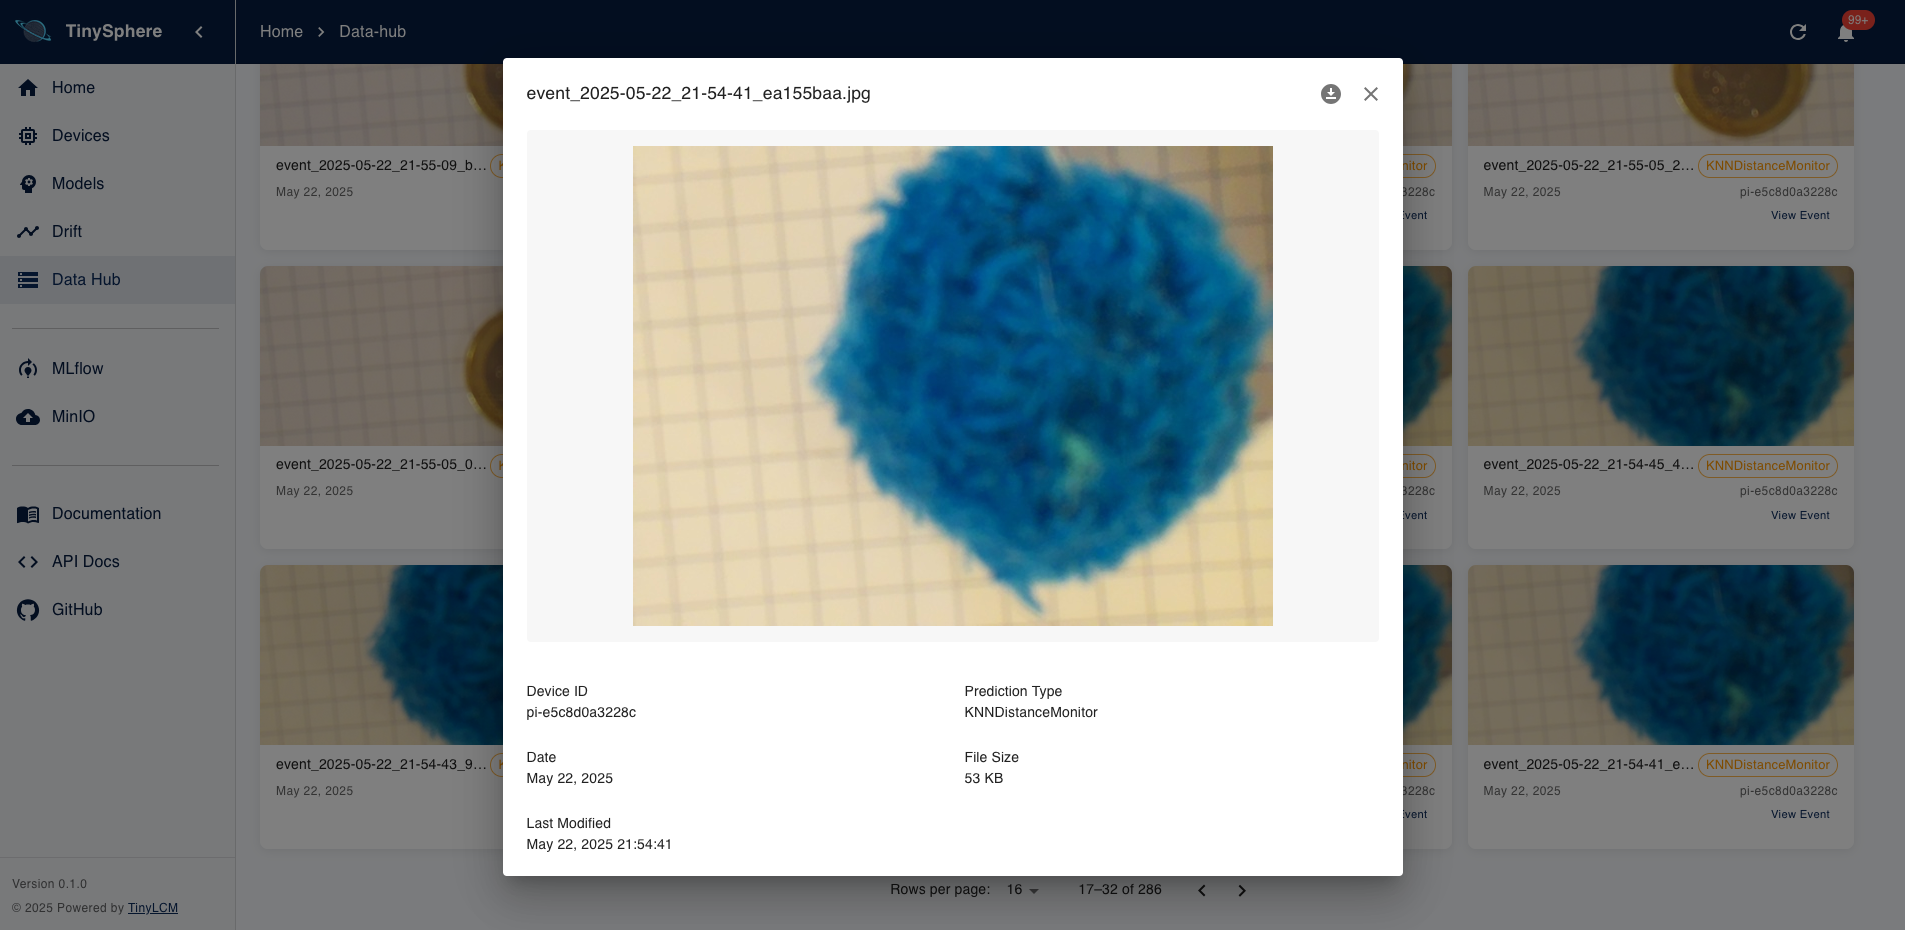
\includegraphics[width=\textwidth]{figs/evaluation/drift_image_exp1_ball.png}
        \caption[Example Drift Image of ``Ball'' (S1)]{Example of a drift-flagged image (object: ``ball'') from  S1, as potentially transmitted to and displayed in the TinySphere Data Hub.}
        \label{fig:drift-image-ball_s1}
    \end{subfigure}
    \hfill 
    \begin{subfigure}{0.49\textwidth}
        \centering
        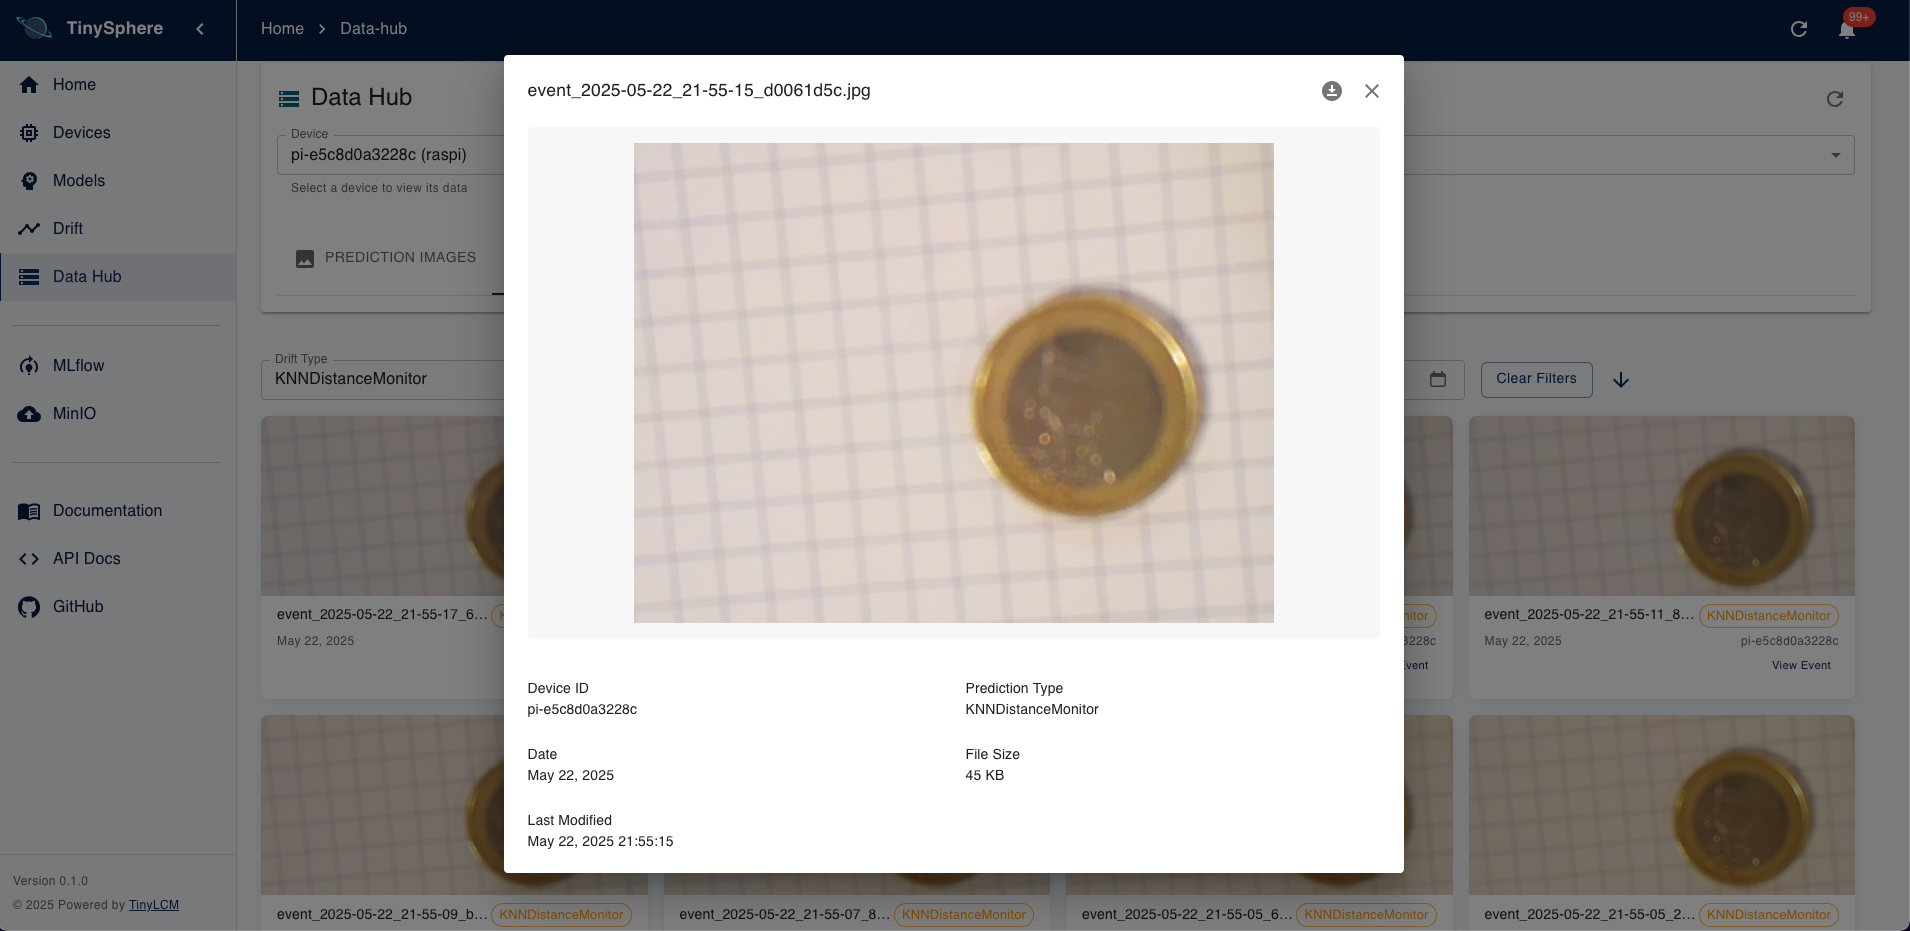
\includegraphics[width=\textwidth]{figs/evaluation/drift_image_exp1_coin.png}
        \caption[Example Drift Image of ``Coin'' (S1)]{Example of a drift-flagged image (object: ``coin'') from  S1, as potentially transmitted to and displayed in the TinySphere Data Hub.}
        \label{fig:drift-image-coin_s1}
    \end{subfigure}
    \caption[Drift Images from S1 (Dual Drift)]{Examples of Drift Images from S1 (Dual Drift) Captured by \gls{tinylcm} and Viewable in TinySphere.}
    \label{fig:combined-drift-images-s1}
\end{figure}

\begin{figure}[htbp]
  \centering
  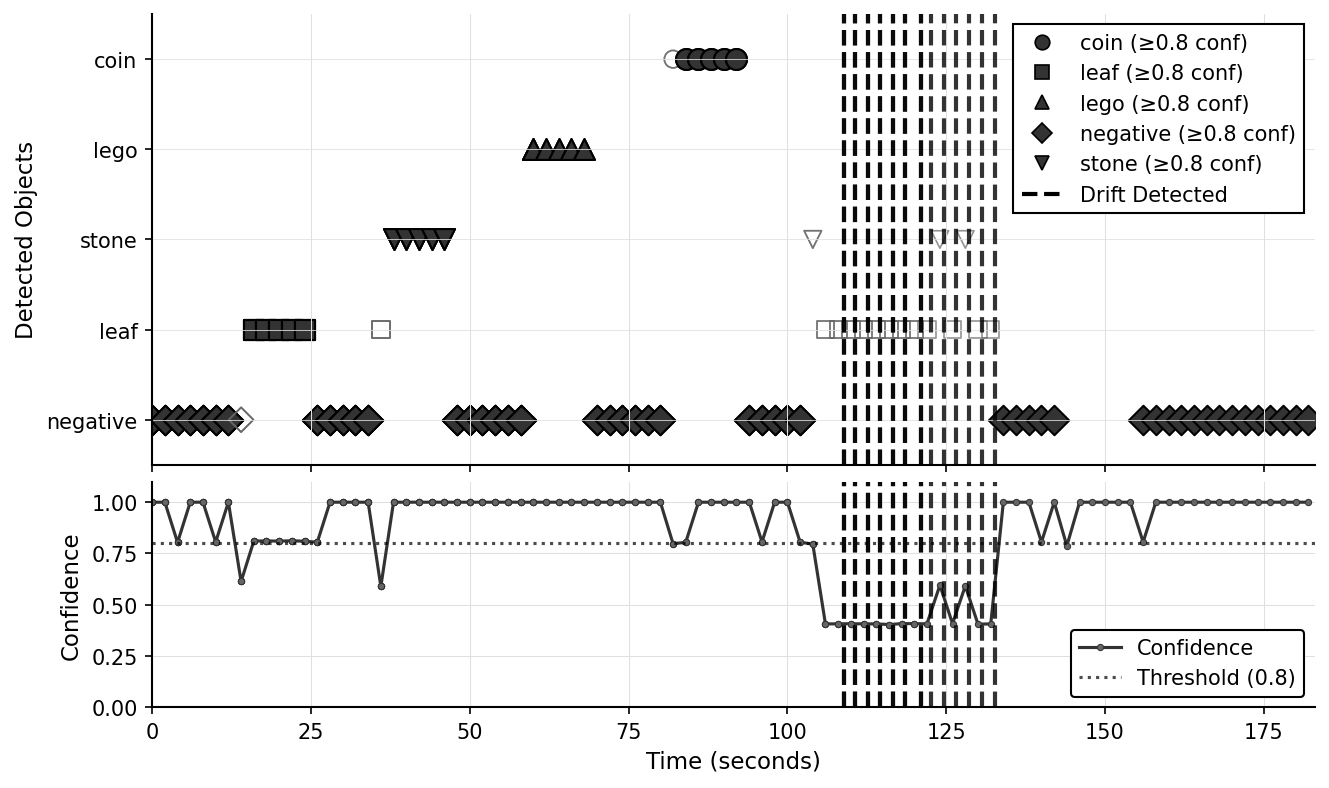
\includegraphics[width=.98\linewidth]{figs/evaluation//drift_ball_timeline.png}
  \caption[Drift Prediction Timeline for Scenario S2 (Single Drift)]{Prediction timeline and drift alarms for Scenario S2 (Single Drift). Visual encoding is the same as in Figure~\ref{fig:timeline-exp1_s1}. In this scenario, ``coin'' is a known class, and only ``ball'' represents a novel drift object.}
  \label{fig:timeline-exp2_s2}
\end{figure}

\begin{figure}[htbp]
  \centering
  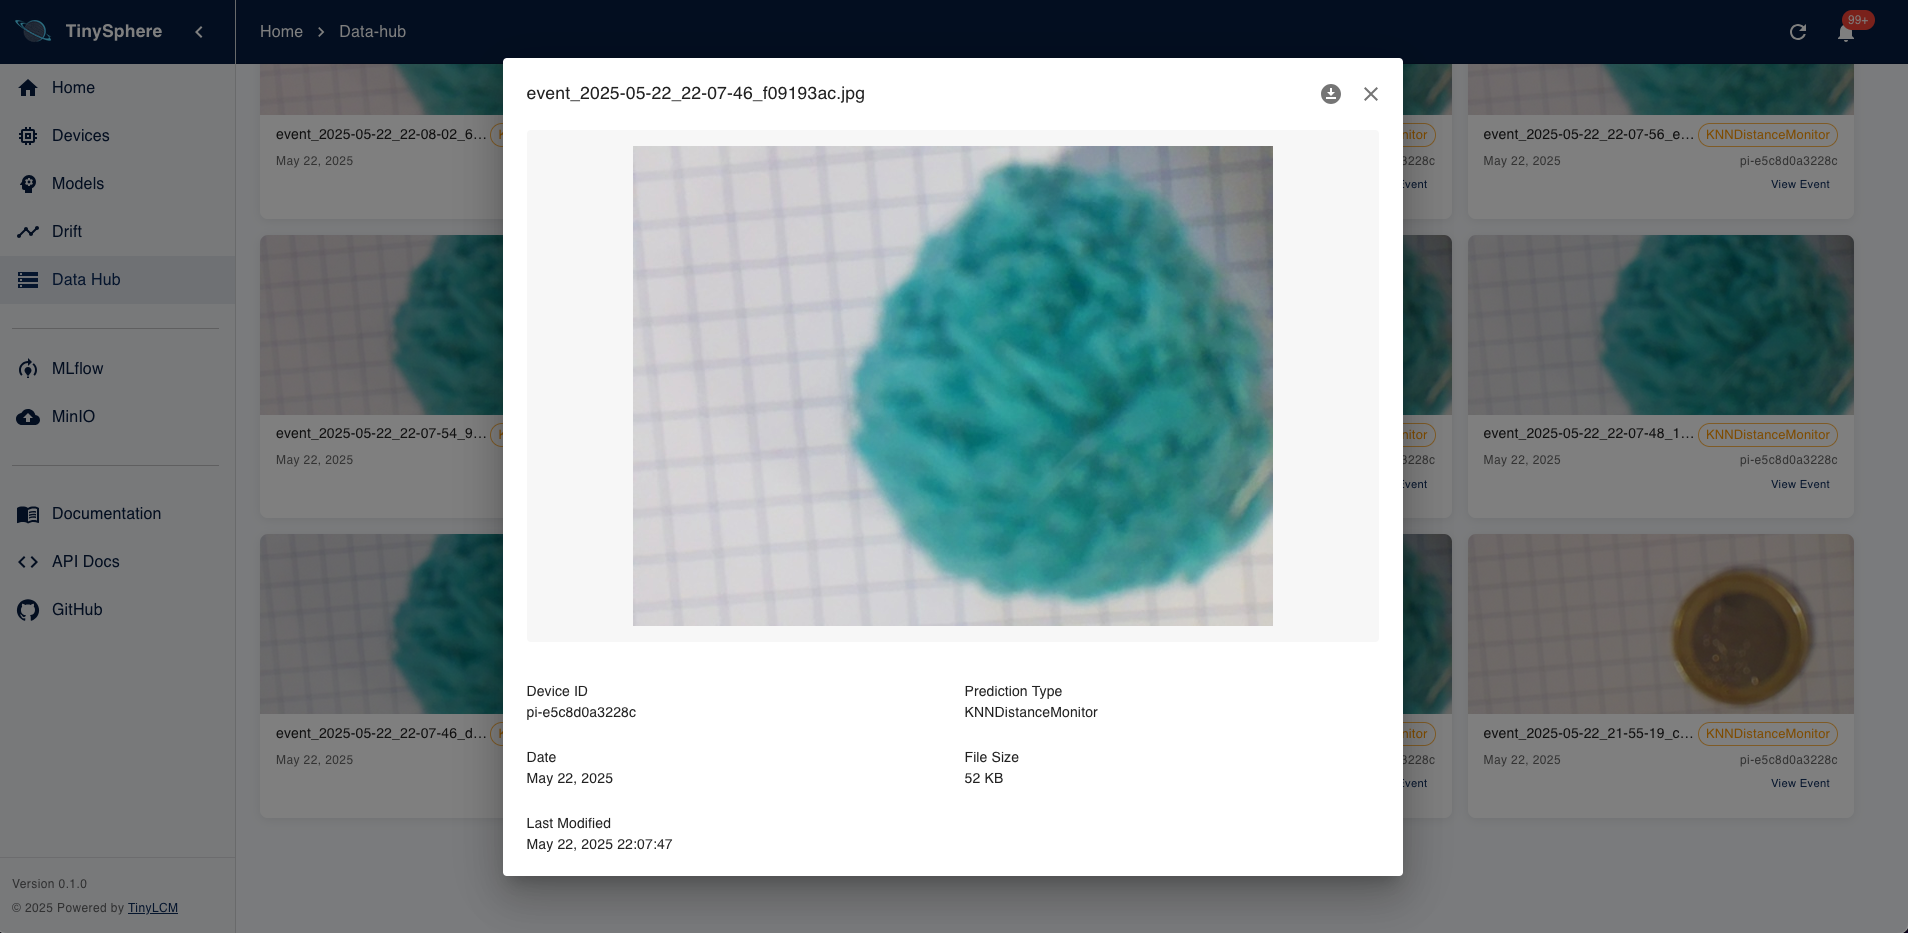
\includegraphics[width=0.59\linewidth]{figs/evaluation/drift_image_exp2_ball.png}
  \caption[Drift Image of Scenario 2 (Single Drift)]{Example of a drift-flagged image (object: ``ball'') from Scenario S2, where ``coin'' was a known class.}
  \label{fig:drift-image-ball-s2}
\end{figure}

\subsection{Quantitative Analysis and Hypothesis Testing (H$_3$)}
\label{ssec:phase2_quantitative_drift_metrics}

To provide a robust assessment beyond qualitative inspection, a quantitative analysis was performed. Each drift check operation was classified into a 2x2 confusion matrix. The results, along with the p-values from the Fisher's Exact Test used to evaluate H$_3$, are consolidated in Table~\ref{tab:drift_detection_combined_results}.

\begin{table}[htbp]
    \centering
    \caption[Quantitative Drift Detection Results and Hypothesis Test for H$_3$]{Summary of drift detection performance and results of the Fisher's Exact Test for H$_3$.}
    \label{tab:drift_detection_combined_results}
    \footnotesize
    \setlength{\tabcolsep}{4pt}
    \begin{tabularx}{\linewidth}{@{} X c c c c r @{}}
        \toprule
        \textbf{Scenario} & \textbf{TP} & \textbf{FN} & \textbf{FP} & \textbf{TN} & \textbf{$p$-value} \\
        \midrule
        S1: Dual Drift (coin \& ball) & 8 & 20 & 10 & 146 & $0.0016$ \\
        S2: Single Drift (ball) & 20 & 6 & 0 & 158 & $8.26\times10^{-22}$ \\
        \bottomrule
    \end{tabularx}
\end{table}

The Fisher's Exact Test for both scenarios yielded statistically significant p-values ($p < 0.05$), as shown in Table~\ref{tab:drift_detection_combined_results}. This confirms a strong, non-random association between the presentation of an untrained object and the triggering of a drift alarm in both cases. Based on this evidence, \textbf{H$_3$ is accepted}.

The acceptance of H$_3$ formally validates the core capability of the \gls{tinylcm} framework: it can detect statistical drift in a manner that is statistically significant. The system can reliably distinguish drift periods from non-drift periods.

However, a separate analysis of the system's sensitivity reveals further insights. The True Positive Rate (TPR) for S1 was 28.6\% (8 out of 28 drift events detected), and for S2, it was 76.9\% (20 out of 26 events detected). This discrepancy highlights a key finding: the system's performance is highly dependent on the nature of the drift and the behavior of the base model.

In Scenario S1, which included the ``coin'' as a second drift object, the sensitivity dropped, and the number of false positives increased. This suggests that the feature representation of the ``coin'' may be less distinct. Consequently, the k-NN distances were likely only marginally or inconsistently higher than the baseline, preventing the Page-Hinkley test from accumulating enough evidence to reliably trigger an alarm. A closer examination of the timeline in Figure~\ref{fig:timeline-exp2_s1} reveals that at the beginning of the ``ball's''s presentation, the base model repeatedly misclassified the novel object as ``lego'' with a high confidence score (approx. 0.8). According to the framework's configuration, the drift check is intentionally bypassed for any prediction exceeding this confidence threshold to save computational resources. Therefore, the poor initial performance of the base model directly masked the drift from the downstream \texttt{KNNDistanceMonitor}. The drift detection only commenced later when the base model's confidence for the misclassification dropped.


\section{Cross-Phase Discussion of Results}
\label{sec:cross_phase_discussion_results}

The empirical evaluation provides key insights into the capabilities and trade-offs of the \gls{tinylcm} framework on a resource-constrained device.

Phase 1 confirmed that \gls{tinylcm}, even with active drift detection, operates within the predefined resource budgets (H$_1$ and H$_2$ accepted). The latency overhead, while statistically significant, remained well below the 50\% threshold. The latency breakdown identified feature processing and \gls{knn} classification as the primary contributors, while the drift check mechanism itself added minimal direct overhead.

Phase 2 provided a quantitative validation of the core drift detection function. By demonstrating a statistically significant correlation between the presentation of untrained objects and the generation of alarms (H$_3$ accepted), the evaluation confirms that the \gls{knn}-based monitoring approach is fundamentally sound. The system is not merely guessing; it is responding to genuine statistical deviations in the feature space.

Synthesizing these findings reveals a central trade-off. \gls{tinylcm} successfully provides a statistically valid drift signal without violating strict performance constraints. However, the Phase 2 discussion highlights that the practical effectiveness of this detection is not constant. It varied significantly depending on the characteristics of the novel object. This implies that while the performance cost of the drift check is low and acceptable (Phase 1), the quality of the resulting detection (Phase 2) is highly dependent on system parameters (like the KNN distance threshold) and the nature of the drift itself. The framework thus offers a tunable, low-overhead mechanism, but achieving high sensitivity for diverse drift types requires careful parameterization and potentially more sophisticated distance metrics, representing a classic trade-off between resource cost, detection robustness, and sensitivity.

\section{Result-Level Threats to Validity}
\label{sec:result_level_threats_validity}

Beyond the general threats to validity inherent in the experimental design (discussed in Chapter~\ref{chp:Research_Design}, Section~\ref{ssec:evaluation_threats_to_validity}), the specific results obtained and their interpretation are subject to further considerations that may impact their generalizability or precision:

\begin{itemize}[noitemsep, topsep=0pt]
    \item \textit{Sensitivity to Drift Detection Parameters and Object Characteristics:} The quantitative results from Phase 2 demonstrated that the detector's sensitivity (TPR) varied significantly between scenarios (28.6\% vs. 76.9\%). This confirms that the framework's performance is highly sensitive to both its internal parameters (e.g., the Page-Hinkley test threshold) and the specific features of the drift object. The parameters were not exhaustively optimized, and the performance on more subtle drift types remains an open question.

    \item \textit{Specificity of ``Drift'' Objects:} The novel objects used (``coin'', ``ball'') were chosen to be visually distinct. While effective for validating the fundamental detection capability, this selection does not cover the full spectrum of concept drift. The framework's performance on more gradual changes or on new objects visually similar to known classes was not explicitly tested.

    \item \textit{Experimental Run Order and Potential Carry-over Effects:} As noted in the methodological reflection in Section~\ref{sec:phase1_results_overhead}, the non-randomized execution order of Phase 1 configurations presents a potential threat to internal validity regarding the precise resource differences observed between the two \gls{tinylcm} configurations.
\end{itemize}
Despite these limitations, the controlled experiments provide strong, quantitative evidence for the feasibility of \gls{tinylcm}'s core functionalities on resource-constrained hardware.

